\documentclass{article}
\usepackage{graphicx}
\usepackage{multicol} % use to multiple column in itemize
\usepackage{float}
\usepackage{setspace}
\usepackage{hyperref}
\setlength{\parskip}{0.5em}

\begin{document}

\title{Clustering}
% \author{Cong Cuong PHAM}

\maketitle

\begin{abstract}
This document introduces some fundamental notions of Clustering.
\end{abstract}

\subsection{Clustering (Unsupdervised)}
\par The goal of clustering is to automatically group similar samples into sets.

Since a clustering algorithm has no prior knowledge of how the sets should be defined, and furthermore, since the clustering process is unsupervised, the clustering algorithm needs to have a way to tell which samples are the most similar, so it can group them. It does this the same way we humans do: by looking at the various characteristics and features of the sample.

\begin{figure}[H]
\centering
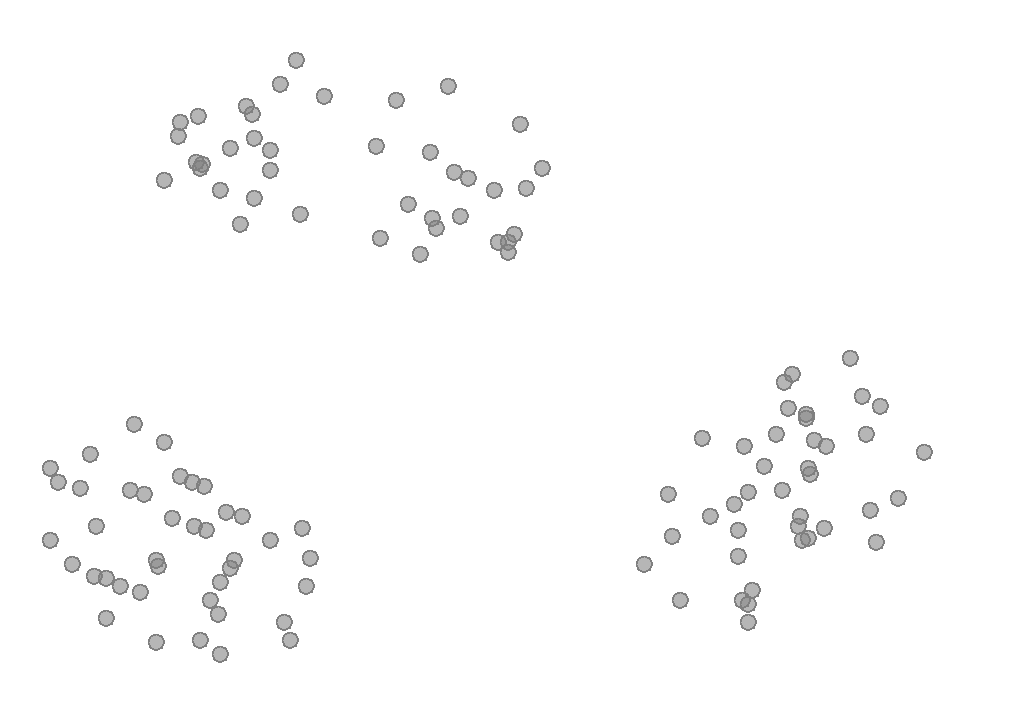
\includegraphics[width=0.6\linewidth]{pic/clustering.png}
\caption{Example of clustering.}
\end{figure}

More examples

\begin{itemize}
    \item Match similar people on a matrimonial site based on their profile question answers.
    \item Based on search history, recommend houses a prospective home-buyer might be interested in considering.
    \item Pinpoint the most likely location for a future earthquake using past earthquake seismic data.
    \item Identify new characteristics shared by different people suffering from the same disease.Calculate an equation to predict the size of a house given its price; or the price of a house given its size.
\end{itemize}

\par There are different types of clustering algorithms, some supervised, some unsupervised. There are even semi-supervised clustering methods as well. In this course, you'll only be dealing only with unsupervised clustering. In other words, the clustering algorithm you will use won't need anything except your raw data. No labels hinting at desired clustering outcome will be provided to the algorithm.

\begin{flushright}
    source: \href{https://courses.edx.org/courses/course-v1:Microsoft+DAT210x+6T2016/courseware/e36e6b45ae5d4032bef2ec557c1ff48f/a8cf8333f6044e9b9a357b7797f282e3/?child=first}{course.edx.org}  
\end{flushright}
\end{document}